\chapter{Regularized Linear Resolution of a One-Compartment Model to Improve the Reproducibility of Perfusion Parameters in CEUS}\label{chapter:IUS}

\section{Abstract}
Contrast-enhanced ultrasound (CEUS) has been proposed to monitor tumor therapy, in complement to size measurements. Estimating reliable perfusion parameters from CEUS studies is essential in order to propose adapted therapy options according to the parameter values. The variability of these parameters was assessed in an ideal case of consecutive test-retest CEUS studies, in a mouse tumor model. The impact of mathematical modeling on parameter variability was investigated on these data. Four models were compared in 32 tumor sub-regions : the log-normal model (LN), the relative LN model (rLN) where parameters of LN are normalized by the parameters estimated inside a reference tissue (RT) region, a linear resolution of a one-compartment model based on the RT (rLin), a modified version of rLin implementing  regularization (rLinReg) to ensure coherent results between the different sub-regions of the tumor. Results show that LN model had highest coefficients of variation. The positive impact of normalization using RT (rLN) was established, showing reduced coefficients of variation. The rLin approach showed large variations especially for flow parameters. Its regularization version, rLinReg, greatly improved parameter reproducibility while providing coherent results between the sub-regions. In conclusion,the rLinReg approach provided the smallest coefficients of variations and should be preferred for estimating perfusion parameters in CEUS.


\section{Introduction}
Reliable quantification of tumor perfusion is a challenging, yet necessary, milestone to reach in order to efficiently monitor tumor growth and treatment efficiency.
Contrast-enhanced ultrasound (CEUS) is a non-invasive tool allowing real-time quantitative vascular imaging: for every sampling time and every pixel in the image, the linearized signal intensity is proportional to the concentration of contrast agent for low concentrations.

Recommendations for the quantification of CEUS studies rely on explicit modeling of time-intensity curves (TICs), e.g.~using a log-normal model~\cite{Dietrich:2012kw}. 
Then, semi-quantitative parameters are usually derived directly from the modeled TIC, e.g.~area under the curve ($AUC$) and wash-in rate ($WIR$). 
These parameters are directly affected by inter-exam changes occurring either in physiology, e.g.~heart rate, blood pressure, or in experimental conditions, e.g.~injected quantity, or injection speed~\cite{Tang:2011fja}.
Controlled injections and compartmental modeling have been proposed to reduce this variability~\cite{Doury:2017fz}. To overcome the issues related to the estimation of a correct arterial input function, the use of a reference tissue (RT) region (e.g.~\cite{CardenasRodriguez:2013em}) has been successfully tested~\cite{Doury:2017fz}. 
In the present study, a linear formulation of the one-compartment model is presented and evaluated. This formulation allows the evaluation of an otherwise unidentifiable parameter, characterizing the RT region, which value had to be set arbitrarily to 0.15. To prove the interest of this new approach, the coefficients of variation of perfusion parameters estimated at a regional scale were compared using four different approaches: 1) the log-normal model (\textbf{LN}), 2) the relative LN model (\textbf{rLN}), where parameters are normalized by the (\textbf{LN}) parameters estimated inside the RT region, 3) a linear resolution of the one-compartment model based on the RT region (\textbf{rLin}), 4) a modified version of \textbf{rLin} implementing  regularization (\textbf{rLinReg}) to ensure a coherent estimation of the ratio between blood flow and blood volume in the RT region when taking into account the different sub-regions in the tumor.


\section{Materials}
\subsection{Animals}
All experiments were conducted in accordance with the institutional guidelines and the recommendations for the care and use of laboratory animals. They were based on a murine model of Murine Colon Carcinoma (CT26). Tumor fragments (20-40 mm$^3$) were implanted 24 days prior to the CEUS acquisitions in the right flank of Balb/C mice. Anesthesia was maintained during the whole acquisition through a face mask delivering 2\% isoflurane in air delivered at a 1 L/min rate. 

\subsection{Image acquisition}
Tumors were imaged in their largest cross-section plane, mice motion was limited using surgical tape securing animal position during and between acquisitions. A controlled injection system was used to inject, at a rate of 4.5 mL/min, a 50 \textmu L bolus of SonoVue (Bracco Suisse SA, Geneva, Switzerland) diluted to 20\%.
Meanwhile, dynamic contrast-enhanced US sequences were acquired using a 15L8W transducer coupled to a Sequoia 512 US system (Acuson, Siemens, Mountain View, CA, USA) in dual-mode, i.e.~anatomical B-Mode along with Contrast Pulse Sequencing (CPS) images. Mechanical index was set to 0.1, dynamic range to 80 dB, and time gain compensation was applied. The frame rate was set to 3 Hz during the first 30 seconds (including the wash-in phase and the beginning of the wash-out phase), and 1 Hz for the remaining time.

For the four mice in the study, four consecutive (test-retest) data-sets were acquired without any modification in the setup. Fifteen minute breaks were observed between acquisitions to ensure the disruption of previously injected micro-bubbles.

\begin{figure*}[ht]
  	\centering
  	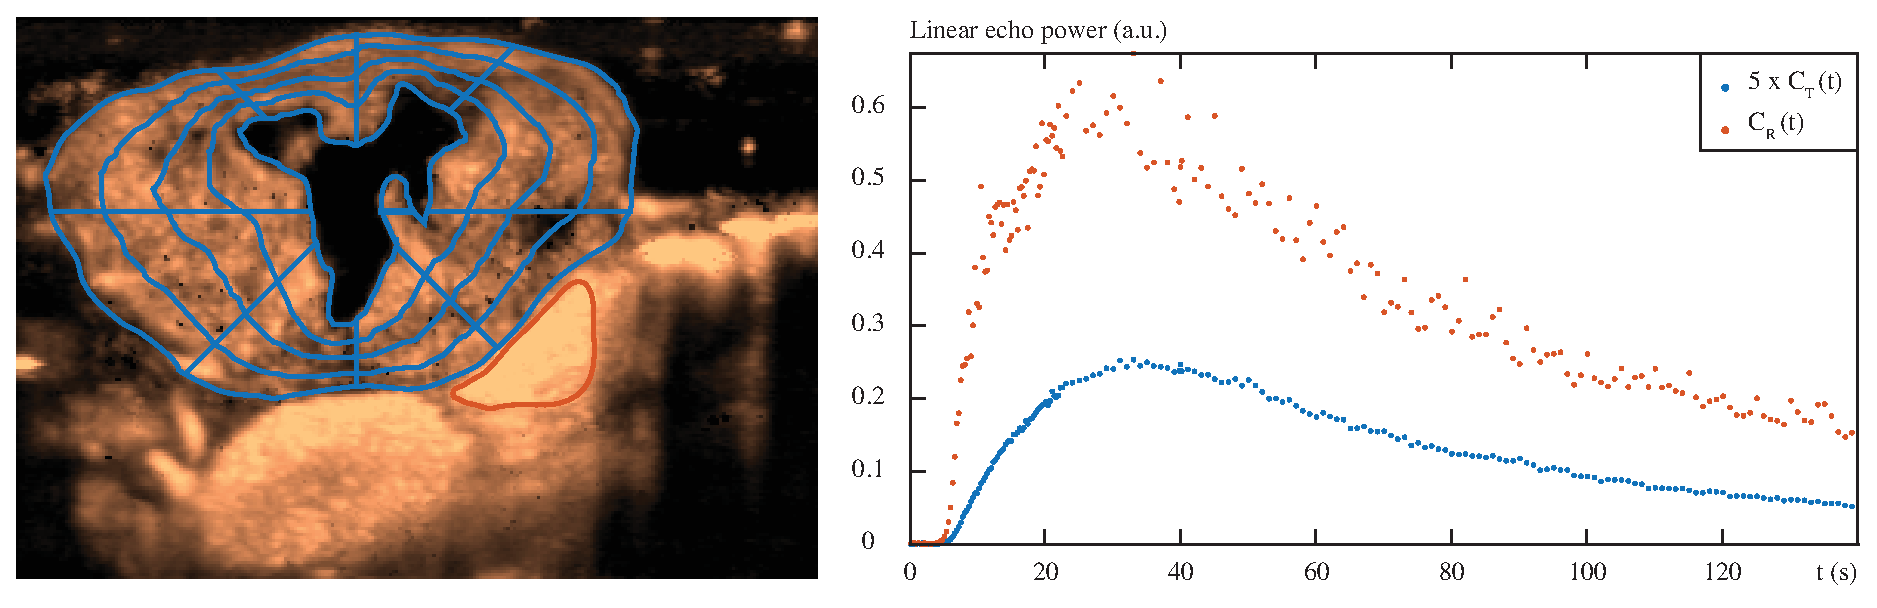
\includegraphics[width=\textwidth]{Ch4_Figure1.eps}
	\caption{Illustration of the data pre-processing steps. Left: The contours of the perfused tumor area have been overlaid on a contrast-enhanced image (in blue color). This area was automatically divided into 4 radial layers and 8 angular sectors as shown by the spiderweb patterns. A RT region (in orange color) was also delineated. Right: Mean TICs associated with the perfused area of the tumor, and the RT.} 
  	\label{fig:Segmentation}
\end{figure*}
\section{Methods}
\subsection{Data pre-processing}
Linear echo-power TICs were calibrated from log-compressed video data using a laboratory-made software.
Both probe and animal motion were assumed negligible for the selected sequences. 

Tumors (hereafter labeled with subscript T) were segmented on the B-Mode images and the non-perfused areas were removed for data analysis.
In order to preserve the signal-to-noise-ratio (SNR) of the TICs while revealing the spatial heterogeneity of the tumor, a regional analysis of the tumor area was performed. 
The perfused tumor region was divided into $N_T = 32$ sub-regions according to 4 radial layers and 8 angular sectors (Figure~\ref{fig:Segmentation}). 
Then mean regional TICs $C_T^i(t)$, for $i=1,...N_T$ were computed. 
As three of the four quantification methods require the selection of a RT region, for each mouse, this RT region (hereafter labeled with subscript R) was chosen to be easily identifiable on the different test-retest studies. 
A muscular region close to the kidney was generally selected, the renal cortex being excluded from the RT region due to the complexity of perfusion patterns observed inside this structure. 

Finally for each sub-region, a time delay parameter, $D_i$, representing the time of arrival of the contrast agent in the considered region, was estimated as follows:
\begin{equation}
D_i = \max_t \frac{\mathrm d^2}{\mathrm dt^2} (C_T^i * W * W),
\end{equation}
where $W$ is an average filter with a fixed width empirically set to 2.0 seconds. 
Using this specific time delay, all regional TICs were registered in time for subsequent analysis.

\subsection{Definition of the four models}
\subsubsection{Log-Normal model (\textbf{LN})}
This method based on the log-normal distribution was recommended by the EFSUMB for quantification of tumor perfusion in clinical studies~\cite{Dietrich:2012kw}.
The TIC inside the $i^{th}$ region of the tumor, $C_T^i(t)$, is fitted according to equation (\ref{eq:LNmodel}):
\begin{equation}
\begin{array}{rcl}
C_T^i(t) &= & \frac{A_T^i}{\sqrt{2 \pi}\sigma_T^i t} \exp \left( - \frac{\left[ \ln(t) - \mu_T^i \right]^2}{2{\sigma_T^i}^2} \right) \textrm{if } t \geq 0,\\ 
&=& \textrm{0 otherwise.}
\end{array}
\label{eq:LNmodel}
\end{equation}
Regional parameters $A_T^i$, $\mu_T^i$, and $\sigma_T^i$  were estimated for each sub-region. 
Semi-quantitative parameters are then derived from the model, including $AUC^i$ and $WIR^i$. These parameters depend, in a non-linear way, on the parameters of the \textbf{LN} model, $A^i$, $\mu^i$, and $\sigma^i$. Relations have been established, both analytically and experimentally, between parameters derived from the \textbf{LN} model and physiological parameters, showing $AUC^i$ is related to blood volume, and $WIR^i$ to blood flow~\cite{Doury:2017fz}.

\subsubsection{Normalized log-normal model (\textbf{rLN})} 
Regional relative parameters: $rAUC^i$ and $rWIR^i$ were derived from the parameters estimated with the (\textbf{LN}) model in the tumor sub-regions ($AUC_T^i$, $WIR_T^i$) and those estimated in the RT region ($AUC_R$, $WIR_R$). 
They were defined as follows:
\begin{equation}
\begin{cases} 
rAUC^i &= AUC_T^i/AUC_R,\\ 
rWIR^i &= WIR_T^i/WIR_R. 
\end{cases}
\end{equation}

\subsubsection{Simple one-compartment model (\textbf{rLin})} 
The resolution of the one-compartment model follows the graphical analysis technique introduced by Patlak et al.~for the quantification of irreversible tracers in PET. 
The method, based on compartmental modeling, estimates blood-related physiological parameters by means of linear regression, assuming the arterial input function (AIF) is known~\cite{Patlak:1983id}.
This linear approach is generalized to reversible tracers~\cite{Logan:1990jg}. 
These approaches have also been adapted to relax the need for blood sampling or AIF measurement and the kinetics inside a RT region was then used (see for instance~\cite{CardenasRodriguez:2013em}).
This resolution was adapted to CEUS data, considering the ultrasound contrast agent is strictly intra-vascular. Considering a one-compartment model to describe flow exchanges inside the tissue, the following equations can be written for each sub-region, $i = 1,\ldots,N_T$:
\begin{equation}
\frac{\mathrm dC_T^i\left(t\right)}{\mathrm dt} = F_T^i.C_A \left(t\right) - \frac{F_T^i}{V_T^i} C_T^i \left(t\right).
\label{eq:Patlak}
\end{equation}
In (\ref{eq:Patlak}) $C_A \left(t\right)$ represents the arterial input function feeding the tissue, while $V_T^i$ stands for the fractional blood volume, and $F_T^i$ for the blood flow in the sub-region $i$.

Considering jointly the TIC inside the RT region and the TICs in the tumor, and assuming a common feeding input for the RT region and the tumor, we have the following set of equations:
\begin{equation}
\left\{ \begin{array}{rcl}
\frac{\mathrm dC_R\left(t\right)}{\mathrm dt} &=& F_R.C_A \left(t\right) - \frac{F_R}{V_R} C_R \left(t\right),\\
\frac{\mathrm dC_T^i\left(t\right)}{\mathrm dt} &=& F_T^i.C_A \left(t\right) - \frac{F_T^i}{V_T^i} C_T^i \left(t\right), \forall i.\\
\end{array}\right.
\label{eq:rLin}
\end{equation}

Rearranging the first equation, $C_A\left(t\right)$ can be isolated and expressed as a function of $C_R\left(t\right)$, and then replaced by its new expression in the $N_T$ following equations, yielding the next system:
\begin{equation}
\left\{ \begin{array}{rcl}
C_A \left(t\right) &=& \frac{1}{F_R} \frac{\mathrm dC_R \left(t\right)}{\mathrm dt} + \frac{1}{V_R} C_R \left(t\right),\\
\frac{\mathrm dC_T^i\left(t\right)}{\mathrm dt} &=& \frac{F_T^i}{F_R} \frac{\mathrm dC_R \left(t\right)}{\mathrm dt} + \frac{F_T^i}{V_R} C_R \left(t\right) - \frac{F_T^i}{V_T^i} C_T^i \left(t\right).
\end{array}\right.
\end{equation}
After integration over time (from 0 to $t$), and definition of the parameters $rF^i = F_T^i/F_R$ , $rV^i = V_T^i/V_R$, and $k_T^i = F_T^i/V_T^i$, the last equations of the system become:
\begin{equation}
C_T^i\left(t\right)=rF^iC_R \left(t\right) + rV^ik_T^i \int_0^t C_R \left(\tau\right)\mathrm d\tau - k_T^i\int_0^t C_T^i \left(\tau\right)\mathrm d\tau.
\label{eq:rLin2}
\end{equation} 
For each sub-region $i$, a sub-system of $N$ linear equations (\ref{eq:rLin2}) is computed, obtained for $N$ successive values of $t$. $N$ is the total number of dynamic frames. Solving this sub-system of $N$ linear equations, the parameters $rF^i$, $rV^i$, and $k_T^i$ can thus be estimated in the least-squares sense. Using this approach, the $N_T$ linear equations corresponding to the different sub-regions are thus solved independently. 

\subsubsection{Regularization of the one-compartment model (\textbf{rLinReg})}
Using the previously described \textbf{rLin} model, $N_T$ different values of $k_R= F_R/V_R$ can be derived, using the estimation of $rF^i$, $rV^i$, and $k_T^i$ and the relation between the four parameters:
\begin{equation}
k_R = \frac{F_R}{F_T^i}\frac{F_T^i}{V_T^i}\frac{V_T^i}{V_R} = \frac{rV^i.k_T^i}{rF^i} \quad \text{for } i = 1,\ldots,N_T.
\end{equation}
As the $k_R$ values do not depend on sub-region $i$, the simple estimation proposed by \textbf{rLin} can introduce some inconsistencies $k_R$  and possible biases in some $rF^i$, $rV^i$, and $k_{T}^i$ values. To solve this issue,
and consider one single value for $k_R$ (whatever the number of sub-regions in the tumor), the regularized approach solves the system of equations  (Eq.~\ref{eq:rLin2}), under the following constraints:
\begin{equation}
\frac{rV^i.k_T^i}{rF^i} = K, \quad \forall i = 1,\ldots,N_T,
\end{equation}
where $K$ is a constant (equal to $k_R$).
The system is solved globally for the $N_T$ sub-regions. Briefly, the value of $k_R$ is successively modified, thus providing a unique least-squares solution for the $3N_T$ parameters ($rF^i$, $rV^i$, and $k_{T}^i$), until the optimization of the fit for the whole set of $N_T$ sub-regions.

\subsection{Data analysis}
For each model, a vector ($\Theta$) of $M$ perfusion parameters ($\theta_m$) was estimated in each tumor sub-region ($i=1,\ldots,32$) of each mouse ($j=1,\ldots,4$) for each repeated acquisition ($k=1,\ldots,4$), providing $512$ results of curve fitting, $\Theta^{ij}_k$, per model. 
The fit quality was assessed quantitatively, using the fraction of modeled information, $FMI$, according to~\cite{Balvay:2005ca}. 

The reproducibility of the perfusion parameters was then deduced for each sub-region of each mouse by computing coefficients of variation $CV(\theta_m)^{ij}$ defined for the four repeated studies, as the ratio between the standard deviation and the mean value $\mu_{m}^{ij}$ of the parameter $(\theta_{m})^{ij}_k$: 
\begin{equation}
{CV(\theta_m)^{ij}} = \frac {\sqrt {\frac{1}{4} {\sum _{k=1}^{4} ((\theta_{m})^{ij}_k- \mu_{m}^{ij})^2}}} {\mu_{m}^{ij}}.
\label{eq:CV}
\end{equation}
Parameters corresponding to poor quality fits ($FMI > 90\% $) were replaced using multivariate imputation by chained equations with the R module \{mice\}~\cite{vanBuuren:2011ica}. This strategy was defined to compute the CV using four values systematically.

Statistical tests were finally applied to compare the CV of the parameters estimated using the four models.
Significant differences in the CV distributions were assessed using the Friedman test and the associated post-hoc analysis for multiple comparisons.  
Distribution means were considered as significantly different when p-values were less than $0.05$.

\section{Results}
\begin{table}[bth]
\begin{center}
\begin{tabular}{lccccc}
\toprule
Model & \textbf{LN} & \textbf{rLN} &\textbf{rLin} & \textbf{rLinReg} \\
\midrule
$FMI$ & 99.3\% & 99.3\%  & 98.8\%  & 98.1\%  \\
$N_{rem}$ & 28  &  28 & 1 & 39 \\
\bottomrule
\end{tabular}
\caption{Median values of $FMI$ obtained for the four models and number of sub-regions $N_{rem}$, out of $512$, for which $FMI <90\%$.}
\label{tab:FMI}
\end{center}
\end{table}

Table~\ref{tab:FMI} shows the median values of the FMI obtained for the four models and the number of regions excluded from further statistical analysis because of bad fit quality. 

\begin{figure}[bth]
  \centering
  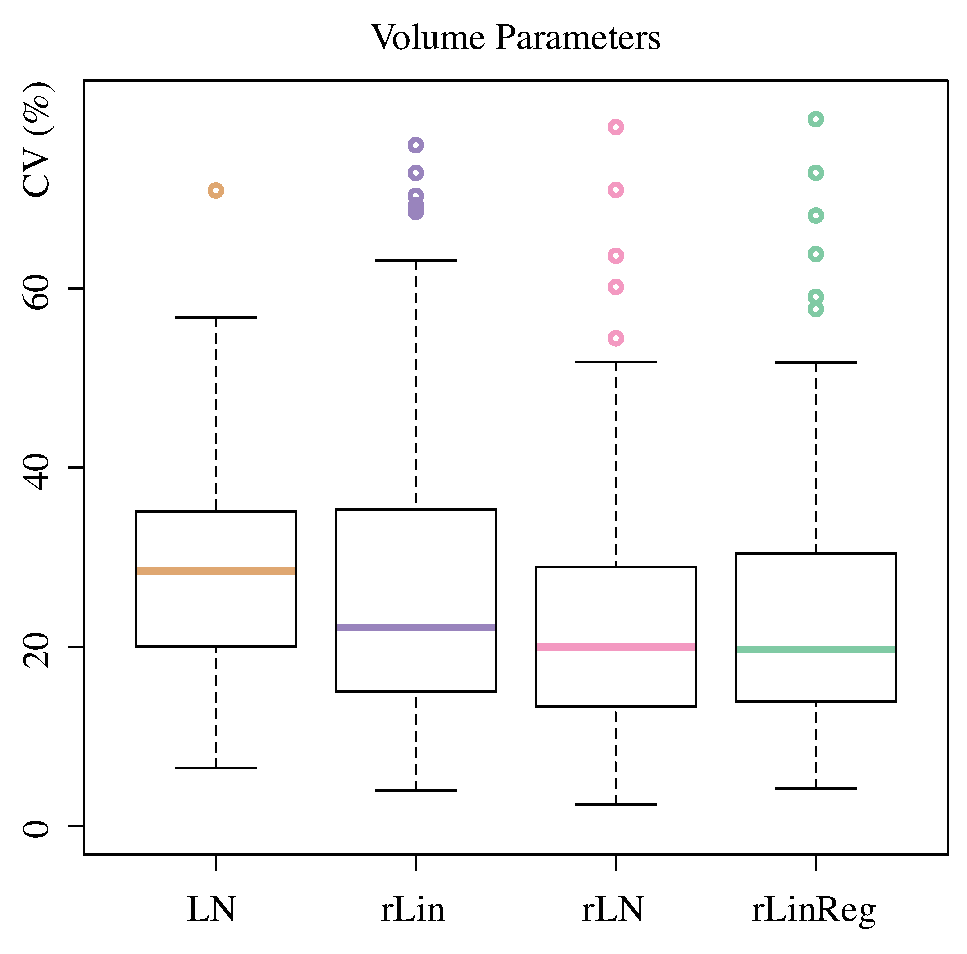
\includegraphics[width=0.49\linewidth]{Ch4_V_CV.eps}
  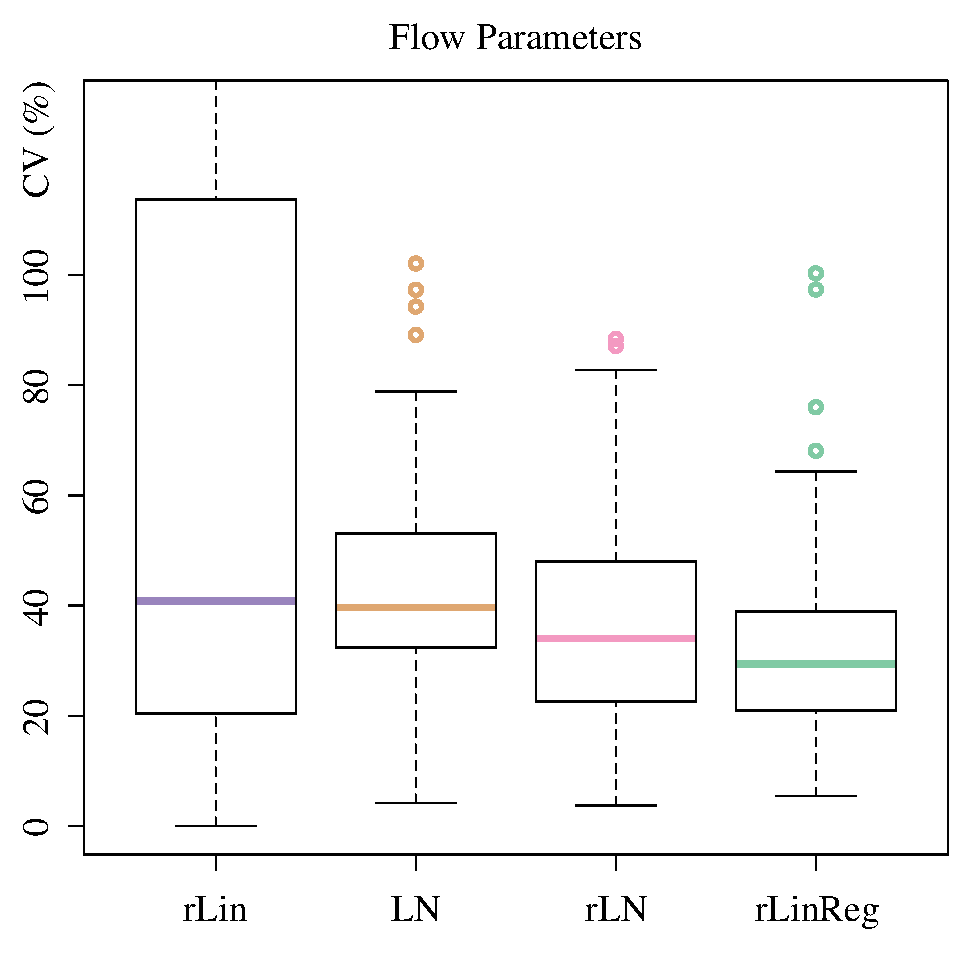
\includegraphics[width=0.49\linewidth]{Ch4_F_CV.eps}
  \caption{Boxplot showing the CV of blood volume  (left) and blood flow (right) estimated with the \textbf{LN}, \textbf{rLN}, \textbf{rLin}, and \textbf{rLinReg} models.}
\label{fig:CV}
\end{figure}

Figure~\ref{fig:CV} displays a boxplot of the $128$ coefficients of variation of blood volume parameters and blood flow parameters obtained for the four models \textbf{LN}, \textbf{rLN}, \textbf{rLin}, and \textbf{rLinReg}. 

\begin{table}
\begin{center}
\begin{tabular}{lcccccc}
\toprule
& \multicolumn{3}{c}{Volume parameters} & \multicolumn{3}{c}{Flow parameters} \\
\cmidrule(l){2-4} \cmidrule(l){5-7}
& \textbf{rLinReg} & \textbf{rLin} & \textbf{rLN} & \textbf{rLinReg} & \textbf{rLin} & \textbf{rLN} \\
\midrule
\textbf{LN} & \textbf{0.001} & 0.1 & \textbf{0.003} & $\mathbf{7 \times 10^{-6}}$ & 0.96 & 0.74 \\
\textbf{rLN} & 0.995 & 0.73 & & $\mathbf{5 \times 10^{-4}}$ & 0.49 \\
\textbf{rLin} & 0.52 & & & $\mathbf{8 \times 10^{-7}}$ \\
\bottomrule
\end{tabular}
\caption{p-values obtained in the post-hoc analysis of the Friedman test. Significant results ($\mathrm p < 0.05$) in bold.} 
\label{tab:pVal}
\end{center}
\end{table}

The p-values obtained after the post-hoc analysis of the Friedman test are shown in Table~\ref{tab:pVal}, significant differences in parameter distributions are emphasized in bold.

In terms of blood volume parameters, the \textbf{LN} model is the most variable with a median value of the coefficient of variation (CV) equal to 28.5\%. 
Using the \textbf{rLin} model, the median CV tends to be lower (22.2\%), however the difference is not statistically significant. 
Models \textbf{rLN} and \textbf{rLinReg} yield significantly more reproducible blood volume parameters than \textbf{LN}, with median CV values of 20.0\% and 19.7\%, respectively. 
For the blood flow parameters, models \textbf{rLin} and \textbf{LN} appear to the most variable parameters with medians of CV equal to 40.8\% and 39.6\%, respectively. 
The \textbf{rLN} model tends to yield lower CV, with a median value of 34.1\%.
Finally the mean CV of blood flow using the \textbf{rLinReg} model is equal to 29.4\%. It is significantly lower than the CV of blood flow obtained with the three other models.

\section{Discussion}
The number of sub-regions was chosen to reveal some spatial heterogeneity in the vascular network of the tumor, while ensuring regions were large enough to guarantee reasonable signal to noise ratios in regional TICs. 
Increasing the number of regions would reveal spatial heterogeneity more finely, at the expense of the accuracy of the estimates.

Both physiological and experimental variations get in the way of accurate quantification and exam comparison, affecting blood circulation, as well as measurements accuracy~\cite{Tang:2011fja}.
The semi-quantitative parameters of the \textbf{LN} model, recommended for tumor quantification, were found highly sensitive to inter-exam changes in our study and resulted in the least reproducible parameters. 
 
When compared to the \textbf{LN} model, the normalized version, the \textbf{rLN} model reduces the variability of parameters. If the reduction of variability for blood flow parameters was not statistically significant, it was significant for blood volume parameters. Thus normalization using a RT region has a real potential to improve exam comparison.

Similarly to the \textbf{rLN} approach, the \textbf{rLin} model uses the RT region, but in addition, it assumes a one-compartment model to describe contrast exchanges between large vessels and micro-vascular areas in tissue.
The first resolution method, which was tested in the present study and proposes to estimate three unknown parameters per sub-region, yields highly variable parameters, especially in terms of blood flow. However, the median CV of blood volume was  reduced when compared to  $AUC$ CV, estimated with the \textbf{LN} model.
This method was implemented in a naive way, resulting in inconsistent values of parameter $k_R$ in the different tumor sub-regions. 

The \textbf{rLinReg} model was built to overcome these inconsistencies, ensuring a single value of $k_R$.
Enforcing a common value of $k_R$ in sub-regions comes down to impose a fixed ratio between the first and second terms of Eq.~\ref{eq:rLin2}.
The number of degrees of freedom was thus reduced. 
The combined use of normalization through a RT region and regularization respects the compartmental modeling paradigm while yielding the most reproducible parameters in our study.

\section{Conclusion}

Using the \textbf{LN} model, derived parameters have high coefficients of variation. 
The positive impact of normalization using a reference tissue region on parameter reproducibility was established. 
The \textbf{rLinReg} approach takes into account the different sub-regions involved in the quantification, yielding a single value of parameter $k_R$ common to all tumor sub-regions. 
In addition, this spatial regularization significantly reduces coefficients of variations of the blood flow parameter and should therefore be preferred to estimate spatially-distributed perfusion parameters.